In this chapter details are provided about the methodology used in the present work to implement an overset grid solver. As a high-level overview, the consideration of overset grids here is based on two main steps: a geometric search and a data communication step. The former generates a tree-based data structure for the mesh nodes which is used to classify the cells around the overset region establishing a receptor-donor relationship. The latter details a conservative high-order approach for the data interpolation and a methodology to impose the interpolated solution throughout the numerical solution.

\section{Overset Grids}

Generally the most common setup for an overset grid system in Computational Fluid Dynamics applications involves a distinct set of meshes: a background and a near-body mesh \cite{DuanThesis2019}. The near-body mesh has a solid body inside and is embedded into a typically much larger mesh, the background mesh. Due to the difference in the physical scale, this configuration eventually provides a considerable processing cost reduction during the simulation in particular for moving boundary applications, since only the near-body mesh has to be re-meshed when the body moves or is deformed as discussed in Refs.\ \cite{Duan2017, Duan2019, Crabill2016}. In order to solve the time advancement of the numerical solution, data must be shared within the outer boundary of the near-body mesh and the overset region inside the background mesh so that it preserves the conservative properties of the fluid. Figure\ \ref{fig:og_setup_fg} illustrates the mesh setup where the near-body mesh is in orange while the background one is illustrated in black.
%
\begin{figure}[H]
	\centering
    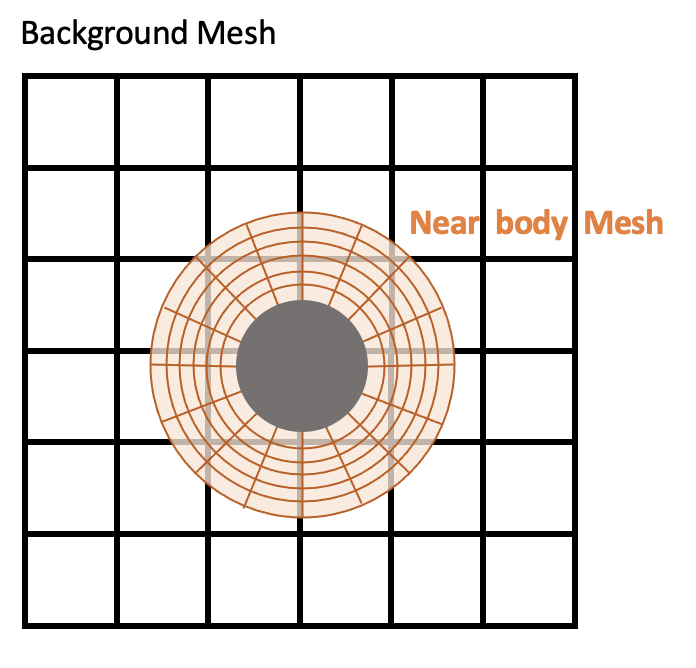
\includegraphics[height=8.0cm]{figs/overset/overset_setup.png}
    \caption{Overset meshes setup: background mesh in black and near-body mesh in orange.}
    \label{fig:og_setup_fg}
\end{figure}

\section{Overset Assembly}
\subsection{Geometric Search}

The definition of a receptor-donor relationship is necessary to communicate data from cells in the background mesh 
to nodes over the external boundary in the near-body mesh. Additionally, some cells in the background mesh may be completely overlapped by the near-body mesh domain and, thus, a procedure to remove these cells from the solver iterations should be performed. This procedure is commonly referred as the hole-cutting process \cite{Crabill2016, Duan2017}. 

In order to simplify both applications, two types of cells are defined: fringe cells and hole cells. Fringe cells will receive, communicate and process data during the solver iterations, while hole cells are skipped with no equation being solved. Hole cells are background cells which are fully emerged at the overset region between the meshes. Thus, the hole cell area solution is only calculated at the near-body mesh cells that overlap it.

\begin{figure}[H]
	\centering
	\subfigure[][]
	{
        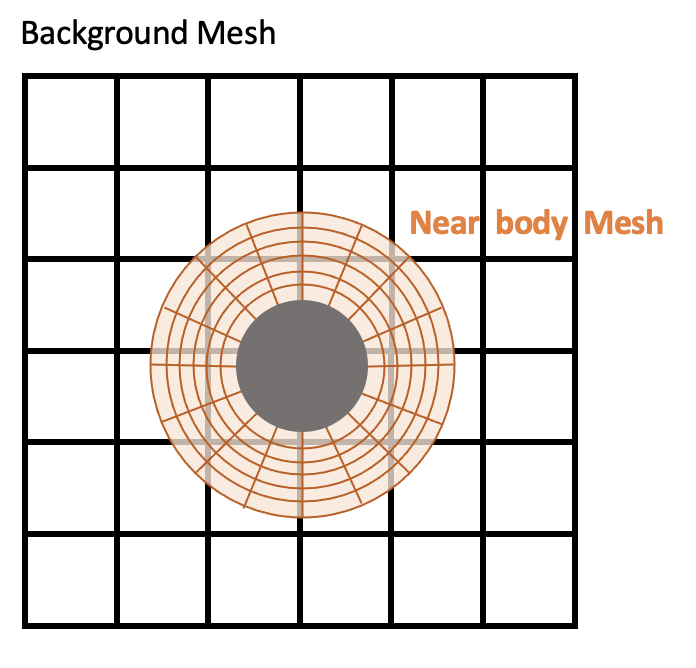
\includegraphics[height=6.0cm]{figs/overset/overset_setup.png}
		\label{fig:og_setup}
    }
    \subfigure[][]
    {
		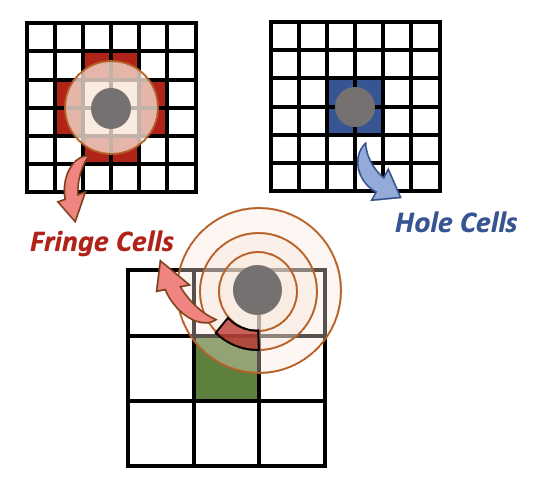
\includegraphics[height=6.0cm]{figs/overset/fringe_hole_cells.png}
		\label{fig:fhcells}
    }
    \caption{Overset grid setup and cell type definitions for a illustrative cylinder example.}
    \label{fig:overset_setup}
\end{figure}

Figure\ \ref{fig:overset_setup} illustrates the setup of background and near-body meshes and the location of some fringe and hole cells. Figure\ \ref{fig:og_setup} shows the overset meshes setup with the near-body mesh in orange and the background mesh in black. Figure\ \ref{fig:fhcells} illustrates the definition of the cell types where the fringes (in red) are used to interpolate solution while holes (in blue) bypass the solver. The green cell is the same fringe cell in red as before, but changed to emphasize near-body fringes. Note that no hole cells are defined for the near-body mesh which means that the solution is calculated for all of its cells at each time step. However, the fringe cells can exist in both meshes and used as donor or receptor for the data communication.

% background vs near-body
% how to structure the connectivity: 
% 1) build a tree structure for both near-body and background meshes
% 2) for each near-body mesh cell at its outer boundary:
%     2.1) for each flux point at an outer boundary edge
%     2.1.1) find the nearest background mesh node using the kd-tree look up
%     2.1.2) given the neaerest node, loop for the background mesh cells that own this node and find in which cell the flux point is inside
%     2.1.3) flag this background cell as a fringe and stores its cell id as donor at the flux point object 
% 3)
% 4) for each fringe cell at the background mesh:
%     4.1) for each flux point at an outer boundary edge
%     4.1.1) find the nearest background mesh node using the kd-tree look up
%     4.1.2) given the neaerest node, loop for the background mesh cells that own this node and find in which cell the flux point is inside
%     2.1.3) flag this background cell as a fringe and stores its cell id as donor at the flux point object 

% IMPROVE THIS PART, MAYBE CHANGE THE INITIAL PART TO SOMETHING LIKE: in order to classify the cells in fringes and holes, firstly we need a methodology that localizes where is the overset region and how to connect one mesh to another
The geometric search problem applied to the context of overset grids aims to define an efficient manner of finding which cell in the donor mesh embeds a specific coordinate in the receiver mesh. In the present work, the kD-tree algorithm described in Ref.\ \cite{Bentley1975} is used for this purpose requiring a tree data structure for the node vectors in both meshes. This tree representation is well suited for the application due to its logarithmic time complexity, which essentially yields a splitting of the domain by half in each search step, according to Ref.\ \cite{Skrodzki2019}. Figure\ \ref{fig:kdtree} illustrates the tree structure in the fluid domain where the dots represent the cell vertices, the blue lines are the x-axis splits of domain, and the orange lines are the y-axis splits of domain. The kD-tree algorithm is built upon all cell vertices and the Fig.\ \ref{fig:kdtree} is only illustrating some vertices for the sake of simplicity. For each split, the median value of one axis is selected so that the nodes in tree structure split the domain in half at each tree depth. 
% KD-TREE
\begin{figure}[H]
	\centering
	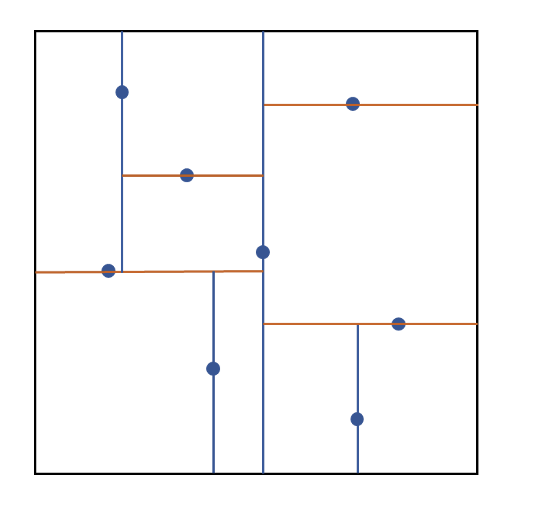
\includegraphics[height=7.0cm]{figs/overset/kdtree.png}
    \caption{kD-tree geometrical view for a given set of points.}
    \label{fig:kdtree}
\end{figure}

The kD-tree structure is build for both the background and near-body nodes and a look-up method of finding the nearest node to a given coordinate is implemented over the tree data structure. The look-up in the kD-tree is done recursively and can be described, for 2-D, in the steps:

\begin{itemize}
  \item A target coordinate is given.
  \item Select a dimension sequentially in alternate cycles between $x$ and $y$. The nodes of the kD-tree are chosen as the approximate median value of the kth-coordinate of the given domain following this alternate dimension cycles. Therefore, at each kD-tree searching step approximately half of the nodes are eliminated from candidate. 
  \item Initially, select the root node as candidate for the nearest node of the testing mesh to the target node.
  \item Calculate the distance between the candidate and the target and store it as the current radius that limits the area where the nearest node can be, as shown in Fig.\ \ref{fig:kdtree_radius_test}.
  \item Compare the selected axis value of the target with the candidate node and check whether the candidate coordinate satisfy the conditions:
  \subitem $target_{k-axis} \leq candidate_{k-axis}$ OR $(target_{k-axis} - radius) < candidate_{k-axis}$
  \subitem $target_{k-axis} >  candidate_{k-axis}$ OR $(target_{k-axis} + radius) > candidate_{k-axis}$
  \item If the first condition is satisfied, repeat the search process with the candidate's right child as the new candidate.
  \item If the second condition is satisfied, repeat the search process with the candidate's left child as the new candidate. 
  \item Compare the minimum distances from both outputs from the left and right sides and finally determine the nearest node to the target.
\end{itemize}
% KD-TREE Radius test
\begin{figure}[H]
	\centering
	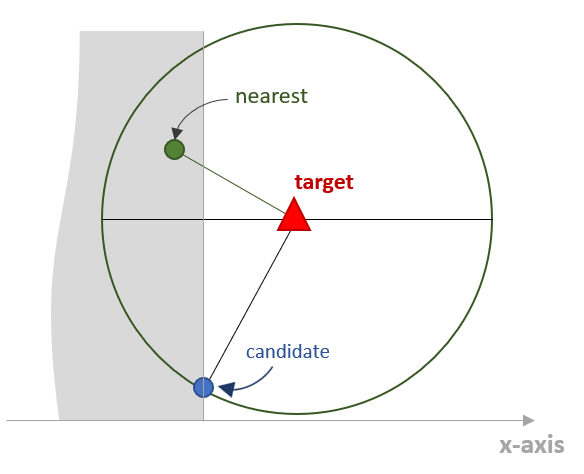
\includegraphics[height=7.0cm]{figs/overset/kdtree_radius_test.png}
    \caption{kD-tree radius test.}
    \label{fig:kdtree_radius_test}
\end{figure}

\subsection{Receptor-Donor Connectivity}

% IMPROVE: generalizes this part to consider not only flux points but any of SD set of points and then states that we are using only for flux points (maybe it should be done only at the data communication section).
The Spectral Difference method, selected in the present work as the spatial discretization method for the governing equations, defines a specific set of points to interpolate the flux vector within the cell domain. Some of these flux-points are located at the cell interfaces and are used to correct the flux discontinuities between neighboring cells. In particular, at the outer and inner boundary interfaces, since the cells at these locations have no neighbor cells, ghost cells are generated containing a mirror of the interface flux-points of the boundary cells. The flux points of the ghost cells are the target coordinates used in the geometric search to map the fringe and initial hole cells. 
% MISSING figure with the types of receptor-donor connectivity (element-based and interface-based)
% references!

At the end of the geometric search process of the boundary flux-points, the nearest node from the donor mesh is found and an additional step is necessary to determine whether the cell, that owns the nearest node, in fact embeds the flux-point. For each cell candidate, a loop throughout its edges is done checking whether the receiver node is inside the candidate cell by validating the sign of the cross product between the edge and the target node, as illustrated in Fig.\ \ref{fig:embeding_cell}. The donor-receiver neighborhood in the physical space is shown in Fig.\ \ref{fig:dr_relation}.
%
\begin{figure}[H]
	\centering
	\subfigure[][]
	{
        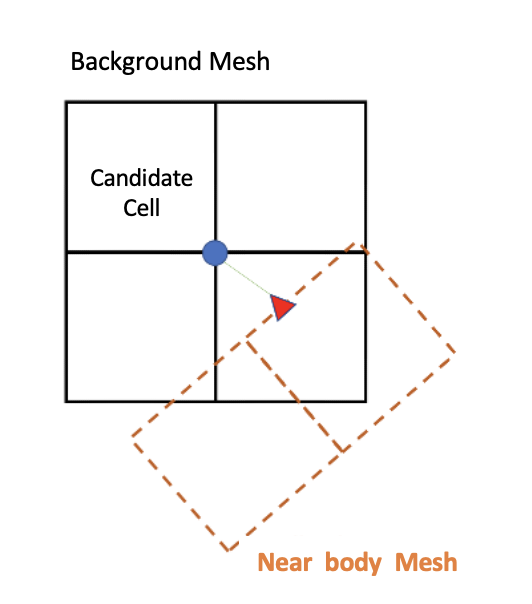
\includegraphics[height=6.0cm]{figs/overset/donor_receiver.png}
		\label{fig:dr_relation}
    }
    \subfigure[][]
    {
		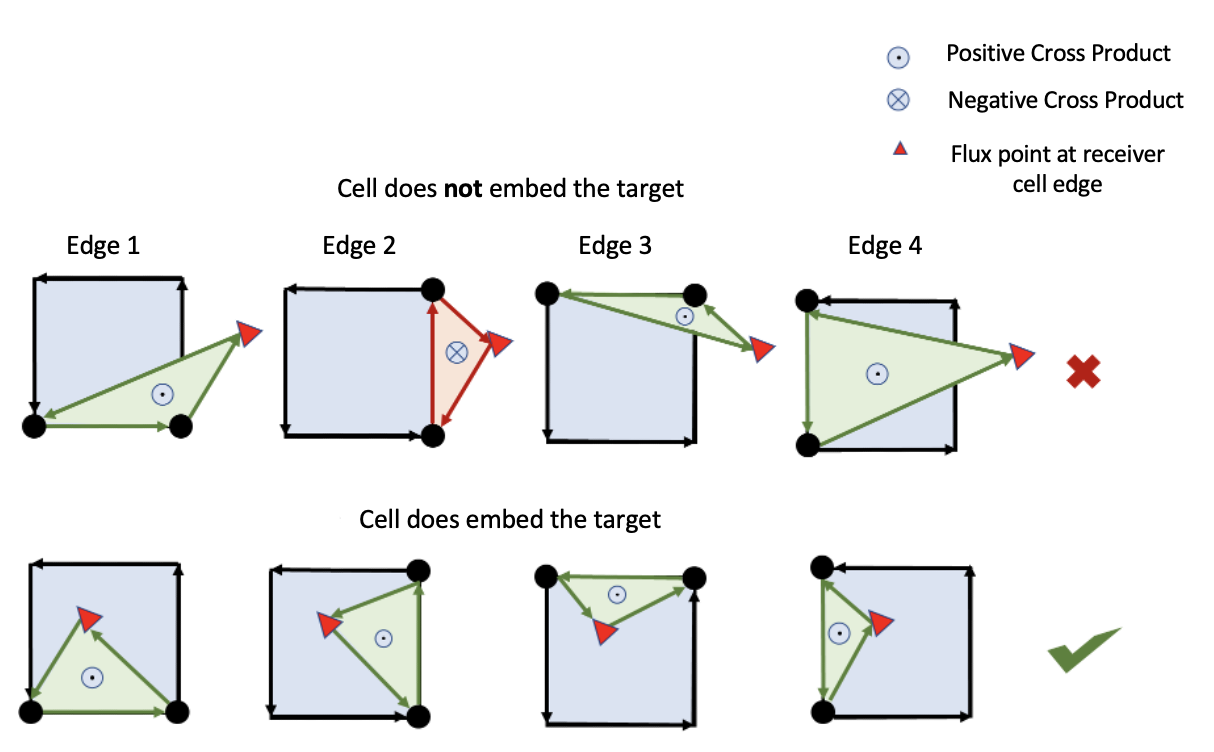
\includegraphics[height=6.0cm]{figs/overset/embeding_cell.png}
		\label{fig:embeding_cell}
    }
    \caption{Donor cell searching procedure given the target node (red triangle) and the nearest donor node (blue circle). The failed test is done over the left bottom cell and the successful test over the right bottom cell.}
    \label{fig:geometric_search}
\end{figure}
%
If all the cross product signs are positive over the counter-clockwise direction, the cell candidate is embedding the flux-point and a fringe flag is attributed to this cell. The fringe cells are determined for the background mesh by applying this search process for each flux point in the ghost cells at the external boundary of the near-body mesh. Moreover, for the near-body mesh, the fringes are determined from the flux points at the inward facing edges of the background mesh fringes as illustrated in Fig.\ \ref{fig:inward_facing_edges}. 
% Inward facing fringe boundary
\begin{figure}[H]
	\centering
	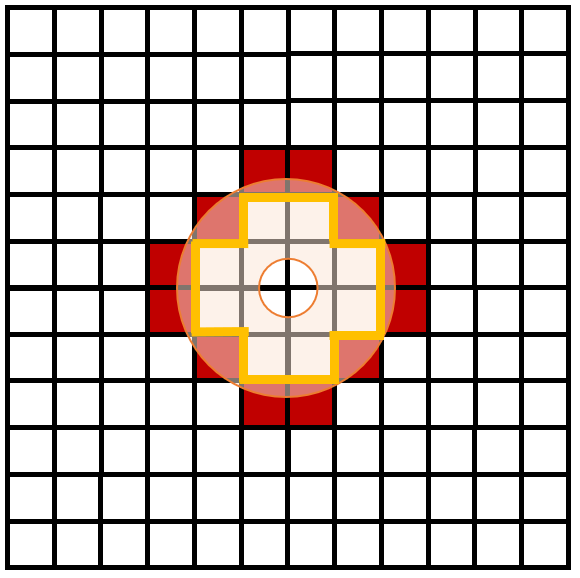
\includegraphics[height=7.0cm]{figs/overset/inward_facing_edges.png}
    \caption{Inward facing edges (in yellow) of the fringe cell circuit in the background mesh.}
    \label{fig:inward_facing_edges}
\end{figure}
% perhaps I could include a second image with the near-body mesh fringes (or I can leave it only for the results)


\subsection{Extension to Curved Meshes}
% explain about the 
The presented donor cell searching procedure uses the vertex nodes of an edge altogether with the target node to determine whether the target node is inside of a candidate cell through its cross product sign. Although it is well -suited for an arbitrary polygon, i.e., it is not restricted to quadrilateral cells, the methodology can result in false positive donor flag classification around curved cells. Figure\ \ref{fig:high_order_mesh_issue} shows a quadrilateral cell with low-order (orange dots) and high-order nodes (blue squares), respectively at Fig.\ \ref{fig:high_order_mesh_issue_a} and \ref{fig:high_order_mesh_issue_b}. The dotted curved lines in Fig.\ \ref{fig:high_order_mesh_issue} illustrates the curvature of the geometry of the cell boundary that is interpolated throughout the high-order nodes. Figure\ \ref{fig:high_order_mesh_issue_c} shows the limitation of cell searching procedure when applied only to the vertex nodes and ignoring the edge curvature which can result in a negative cross product over the low-order edge, even though the target node is indeed inside the cell.
%
\begin{figure}[H]
	\centering
	\subfigure[][]
	{
        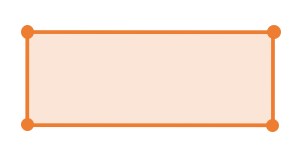
\includegraphics[height=3.5cm]{figs/overset/high_order_issue_p1.png}
		\label{fig:high_order_mesh_issue_a}
    }
    \subfigure[][]
    {
		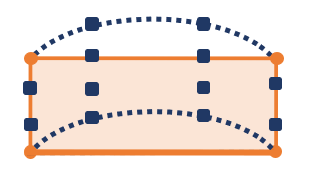
\includegraphics[height=4.0cm]{figs/overset/high_order_issue_p2.png}
		\label{fig:high_order_mesh_issue_b}
    }
    \subfigure[][]
    {
		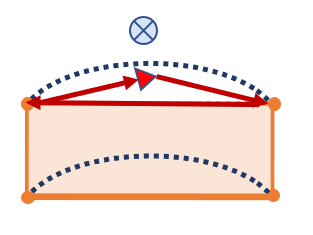
\includegraphics[height=5.0cm]{figs/overset/high_order_issue_p3.png}
		\label{fig:high_order_mesh_issue_c}
    }
    \caption{Cell searching procedure issue for curved cells.}
    \label{fig:high_order_mesh_issue}
\end{figure}

The extension approach includes the high-order nodes over the edges as if the quadrilateral were an arbitrary polygon so that the information of curvature can be considered leveraging the same cell searching procedure as explained in the receptor-donor relationship section. Figure\ \ref{fig:high_order_mesh_extension} exemplifies the sequence of cell searching procedure using the high-order interface nodes (blue squares) and vertices (orange dots). Commonly the enumeration of high-order nodes in the vector of nodes is posterior to the vertices, i.e., the low-order nodes are counted first. This is relevant for this procedure since it considers the counter-clockwise direction as reference for the sign comparison which, then, requires a simple re-enumeration step for the vector of nodes in each edge.
%
\begin{figure}[H]
	\centering
	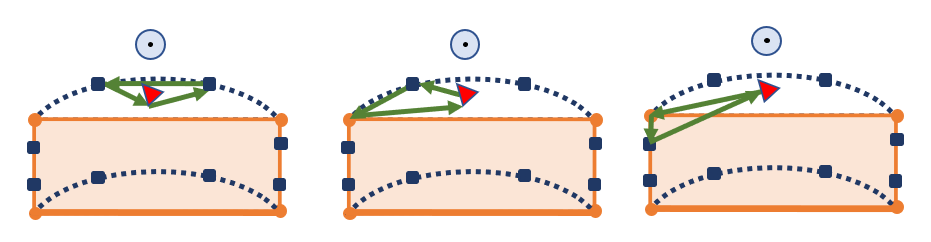
\includegraphics[height=4.0cm]{figs/overset/high_order_extension.png}
    \caption{High-order edges nodes inclusion in the cell searching procedure.}
    \label{fig:high_order_mesh_extension}
\end{figure}

\subsection{Hole-Cutting}
For the hole cells, a random node in the near-body grid is then selected until its donor cell output in the background satisfy the conditions of not being a fringe and being completely overlapped by the near-body mesh. This cell is flagged as a hole cell and it is used as input for a Breadth-First Search (BFS) algorithm which propagates the hole flag for the unmarked cells until all interior cells within the fringe closed circuit are visited \cite{CormenBook2009}. Figure\ \ref{fig:hole_cutting_bfs} shows a sketch of this procedure where the first hole cells are flagged through an inner boundary or random internal node from the near-body mesh. Then, the child of a hole cell is only stacked to be visited in the next iteration if it is not a fringe cell. At last, new ghost cells are created at the fringe-hole interfaces in order to correct the flux normal to its edges by communicating data from the near-body mesh. The same donor-receiver relationship procedure is done to determine which cells at the near-body mesh embeds all flux points in these ghosts as well.
% 
\begin{figure}[H]
	\centering
	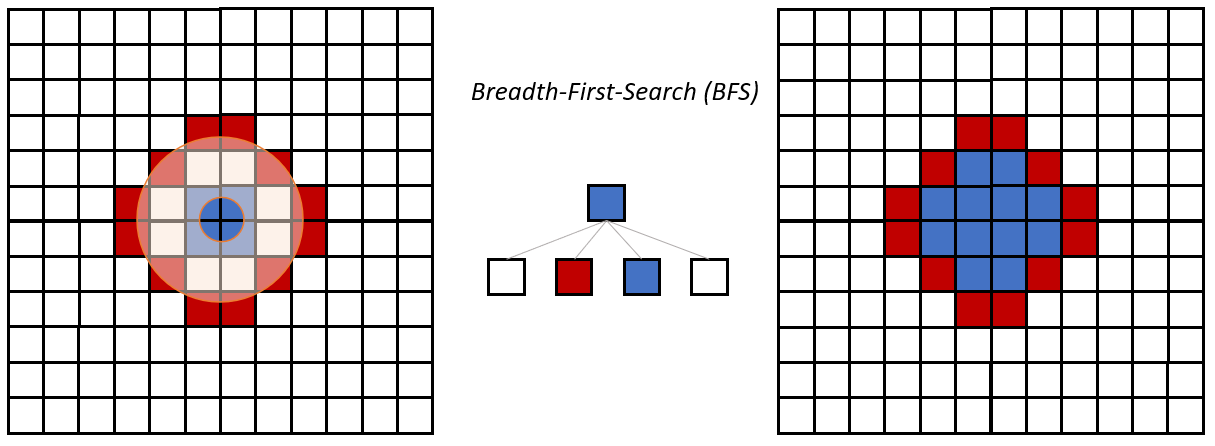
\includegraphics[height=5.0cm]{figs/overset/hole_cutting_bfs.png}
    \caption{Hole-cutting flag (blue) propagation using a Breadth-First Search (BFS) algorithm conditioned by the fringe cell circuit (red).}
    \label{fig:hole_cutting_bfs}
\end{figure}

\section{Data Communication}

\subsection{Data Interpolation}
% explain about the element-based and face-based approaches and which the project uses.
The first methods to consider overset grids were based on low-order solvers restricted to structured meshes as in the NASA's PEGASUS software \cite{Suhs2003}. Moreover, the approach for data communication during these first implementations was developed mostly using a bilinear interpolation which can limit the accuracy order of the interpolated solution. Recently, new data communication methodologies have been developed extending some high-order methods in the FR/CPR framework to overcome the limitations of the bilinear interpolation and additionally to consider unstructured overset grids. In order to provide a conservative high-order data communication, two different approaches were developed firstly for Discontinuous Galerkin type methods: the face-based \cite{Galbraith2013} and the element-based approaches \cite{Nastase2016, Brazell2016}. 
%
\begin{figure}[H]
	\centering
	\subfigure[][]
	{
        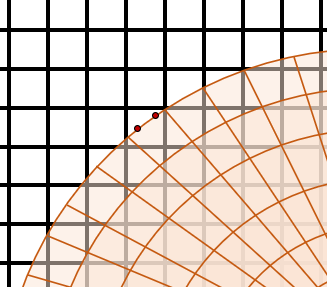
\includegraphics[height=5.0cm]{figs/overset/face_based_approach.png}
		\label{fig:space_transform}
    }
    \subfigure[][]
    {
		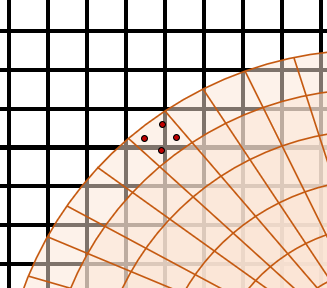
\includegraphics[height=5.0cm]{figs/overset/element_based_approach.png}
		\label{fig:interpolation}
    }
    \caption{Data communication nodes setup at the overset region for face-based and element-based approaches.}
    \label{fig:data_communication}
\end{figure}

In the face-based approach illustrated in Fig.\ \ref{fig:space_transform}, the solution data is interpolated from the donor cells that embed nodes located at the outer boundary faces around the overset region. The interpolated solution is used to calculate the flux at the interface and is applied as a weak boundary condition in the outer boundary. The Riemann solver can, then, be applied to correct the flux in the overset interfaces \cite{Galbraith2013}.

In the element-based approach in Fig.\ \ref{fig:interpolation}, the solution data is interpolated to internal points of the cells located at the outer boundary. Differently to the face-based approach, the interpolated solution here is used to interpolate the solution within the cell domain and is imposed as the solution in the current iteration step \cite{Duan2019}.

For the present work, the face-based approach is used due to its simpler implementation and greater robustness in comparison with the element-based, according to Refs.\ \cite{Galbraith2013, DuanThesis2019}.

\subsection{Standard Space Projection}

The cells in the Spectral Difference method are projected to a standard space where the solution can be represented through a nodal interpolation using specific polynomial basis functions. This standard space transformation is unique for each cell and is defined by the cell Jacobian matrix $J$ which is a function of the computational space coordinates $\xi, \eta$ for curved cells. In the context of data communication, the solution is interpolated from the set of solution points of the donor cell to a target node at the receptor standard space. The target node in the face-based approach is a flux-point whose space coordinates are commonly stored in the computational space of the receptor cell. In order to assemble the data communication, the target coordinates need to be projected from the receptor standard space into the donor standard space so that the solution can be interpolated as illustrated in Fig.\ \ref{fig:space_transform_p1}. 
%
\begin{figure}[H]
	\centering
	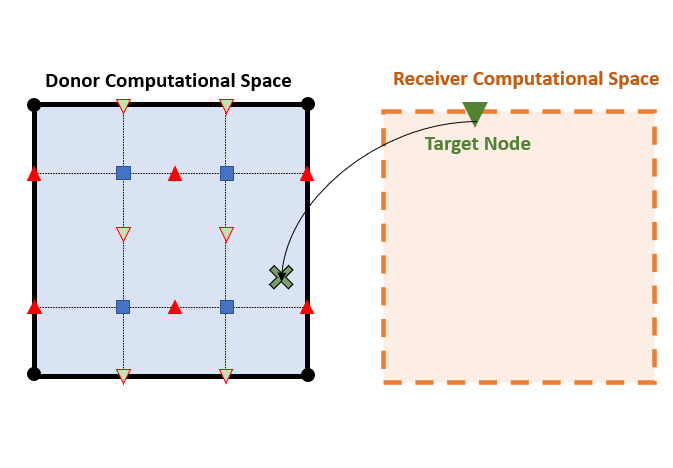
\includegraphics[height=8.0cm]{figs/overset/space_transformation_p1.png}
    \caption{The target node is projected from the receiver to the donor computational space.}
    \label{fig:space_transform_p1}
\end{figure}
%
This coordinate transformation can be done in two steps. First the target coordinate is projected from the receiver computational space to the physical space using Eq.\ \ref{eq_ho_quad_1}. Then, this physical space coordinate is used in Eq.\ \ref{eq_ho_quad_2} to determine the $\xi, \eta$ coordinates in the donor computational space allowing the interpolation of the solution through Eq.\ \ref{eq_sp_lagr} as illustrated in Fig.\ \ref{fig:space_transform_p2}. Note that a non-linear system of equation has to be solved to find the target $\xi, \eta$ coordinates in Eq.\ \ref{eq_ho_quad_2}. In the present work, a Newton-Raphson solver is used where the function is defined by Eq.\ \ref{eq_ho_quad_2} and its derivative through the Jacobian matrix. 
%
\begin{figure}[H]
	\centering
	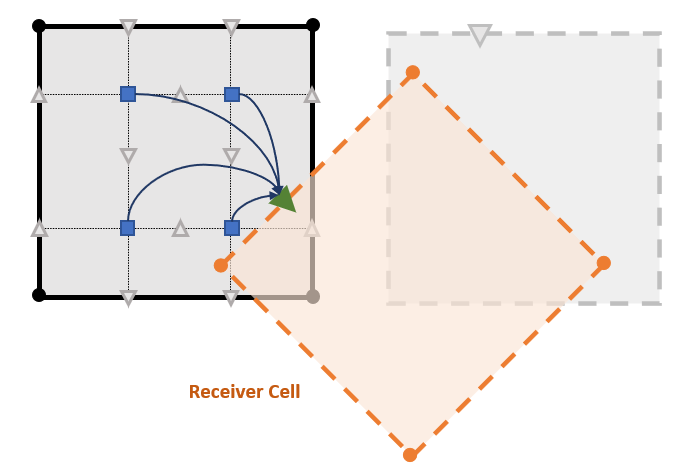
\includegraphics[height=8.0cm]{figs/overset/space_transformation_p2.png}
    \caption{The solution is interpolated to the target coordinate inside the donor computational space.}
    \label{fig:space_transform_p2}
\end{figure}
%
%\begin{figure}[H]
%	\centering
%	\subfigure[][The target node is projected from the receiver to the donor computational space.]
%	{
%        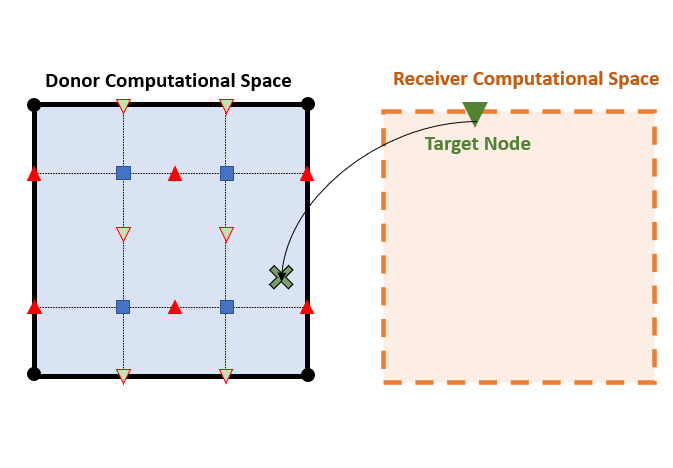
\includegraphics[ height=5.0cm ]{figs/overset/space_transformation_p1.png}
%		\label{fig:space_transform_p1}
%    }
%    \subfigure[][The solution is interpolated to the target coordinate inside the donor computational space.]
%	{
%        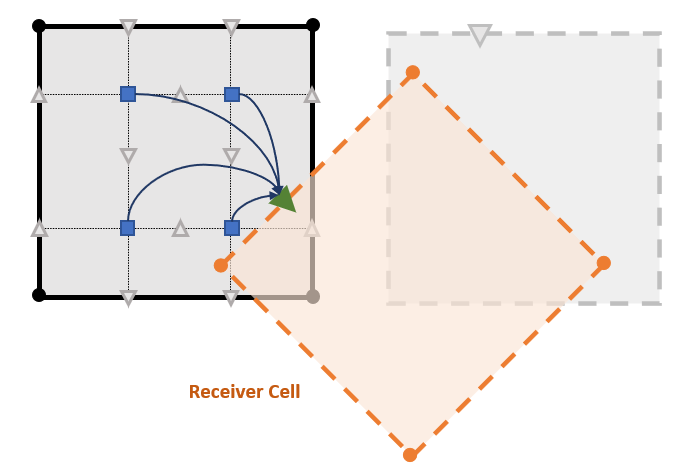
\includegraphics[ height=5.0cm ]{figs/overset/space_transformation_p2.png}
%		\label{fig:space_transform_p2}
%    }
%    \subfigure[][The interpolated solution (arrow) is then projected back to the receiver computational space.]
%	{
%        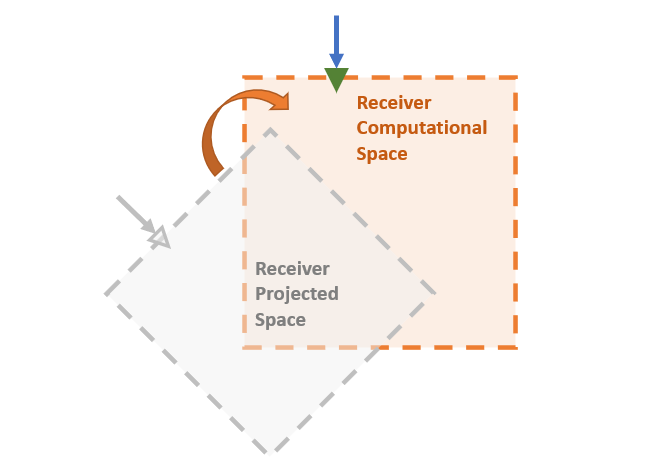
\includegraphics[ height=5.0cm ]{figs/overset/space_transformation_p3.png}
%		\label{fig:space_transform_p3}
%    }
%    \subfigure[][Imposition of the interpolated solution as a weak boundary condition using flux reconstruction.]
%	{
%		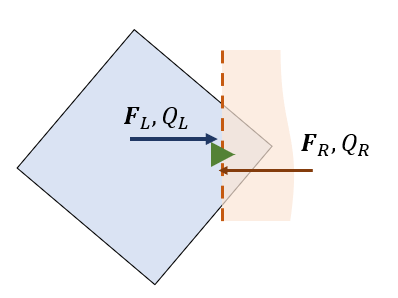
\includegraphics[ height=5.0cm ]{figs/overset/interpolation.png}
%		\label{fig:space_transform_p4}
%    }
%    \caption{Data communication procedure including the space transformation and data interpolation steps.}
%    \label{fig:data_communication_steps}
%\end{figure}
%
For high-order meshes, the Jacobian matrix of the transformation from the physical to the computational space is not constant within the cell domain, but a function of the target $\xi, \eta$ coordinates. Therefore, for each Newton-Raphson iteration, the Jacobian matrix has to be computed with the updated guess of the projected target coordinates. The subscript $R$ stands for receiver and $D$ for donor.
%
\begin{equation}
    \label{eq_ho_quad_1}
   x_{FP_t} = \sum_{m=1}^{(N+1)^{2}}{{L_{R}}^{N+1}_m(\xi_{R_{target}}) {L_{R}}^{N+1}_m(\eta_{R_{target}}) {x_R}_{m}}
\end{equation}
%
\begin{equation}
    \label{eq_ho_quad_2}
  \sum_{m=1}^{(N+1)^{2}}{{L_{D}}^{N+1}_m(\mathbf{\xi_{D_{target}}}) {L_{D}}^{N+1}_m(\mathbf{\eta_{D_{target}}}) {x_D}_{m}} = x_{FP_t}
\end{equation}
%
After the target coordinate is projected to the donor computational space $\mathbf{\xi_{D_{target}}}, \mathbf{\eta_{D_{target}}}$, the solution can be interpolated through Eq.\ \ref{eq_sp_lagr} preserving the same high-order polynomial representation of the solution used by the Spectral Difference method. 
%
\begin{figure}[H]
	\centering
	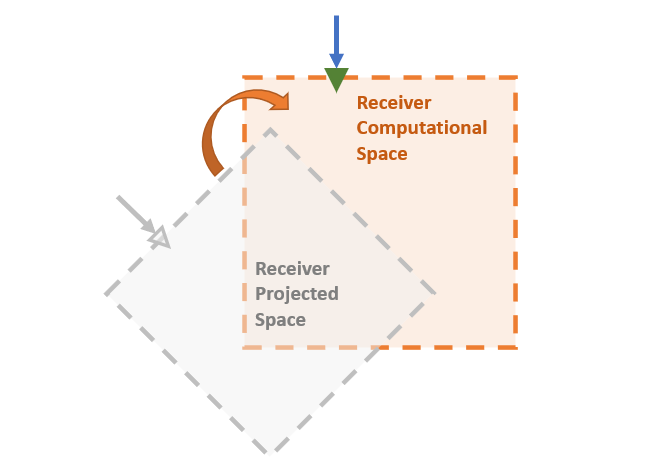
\includegraphics[height=8.0cm]{figs/overset/space_transformation_p3.png}
    \caption{The interpolated solution (arrow) is then projected back to the receiver computational space.}
    \label{fig:space_transform_p3}
\end{figure}

The interpolated solution still lies in the donor computational domain and, therefore, needs to be projected back to the receiver computational domain.  Figure\ \ref{fig:space_transform_p3} illustrates the space projection step from the donor computational space into the receiver computational space. 

First the interpolated solution is projected from the donor computational space to the physical space using the donor Jacobian matrix calculated at the target node. Then, the solution at the physical space is transformed to the receiver computational space through the receiver Jacobian matrix as described in Alg.\ \ref{alg:space_projection}. The interpolated solution in the receiver computational space is imposed as a weak boundary condition for the Riemann solver, i.e., the solution is not imposed to assume the interpolated value, but instead it is used through a Riemann solver in order to reconstruct a continuous flux at the interfaces by the use of Eq.\ \ref{eq_riemann}. The boundary condition is illustrated in Fig.\ \ref{fig:space_transform_p4}.
%
\begin{figure}[H]
	\centering
	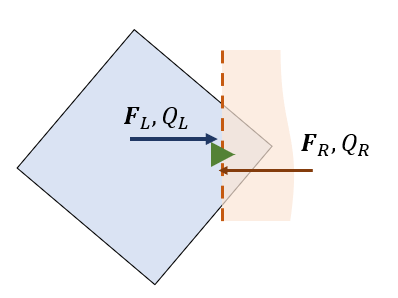
\includegraphics[height=7.0cm]{figs/overset/interpolation.png}
    \caption{Imposition of the interpolated solution as a weak boundary condition using flux reconstruction.}
    \label{fig:space_transform_p4}
\end{figure}
%

\begin{algorithm}
\caption{Pseudo-code for the interpolated solution projection from the donor to the receiver.}
\label{alg:space_projection}
\begin{algorithmic} [1]
\State // Calculate the Donor Jacobian matrix at the target node 
\State $J_{Donor} \gets Donor.CalculateJacobianAtNode(\xi_{D_{target}}, \eta_{D_{target}})$ \\
\State // Transform the solution from computational donor space to the physical space 
\State $Q_{Physical} \gets (\frac{1.0}{J_{Donor}}) Q_{Interpolated}$ \\
\State // Get the receiver Jacobian matrix at the target flux-point 
\State  $J_{Receiver} \gets Receiver.Jacobian(\xi_{D_{target}}, \eta_{D_{target}})$ \\
\State // Transform the solution from the physical space to the computational receiver space 
\State $Q_{Receiver} \gets J_{Receiver} Q_{Physical}$ 
\end{algorithmic}
\end{algorithm}

